%trucs qui clignottent(minipage?)
%enumeration ; ; ; . . .
%\cdot


\section{Introduction}

\subsection{Hybrid systems}
\begin{frame}{What is an hybrid system?}
\begin{center}

\includegraphics[width=0.9\columnwidth]{images/continuous.pdf}
%ajouter photos?
\end{center}
\end{frame}

\begin{frame}{What is an hybrid system?}
\begin{center}
\vspace*{-1.5cm}
\includegraphics[width=\columnwidth]{images/cs.pdf}
%ajouter photos?
\end{center}
\end{frame}

\begin{frame}{A model: the hybrid automaton}
\begin{center}
\begin{columns}[c]
\begin{column}{5cm}
\hspace*{-0.5cm}
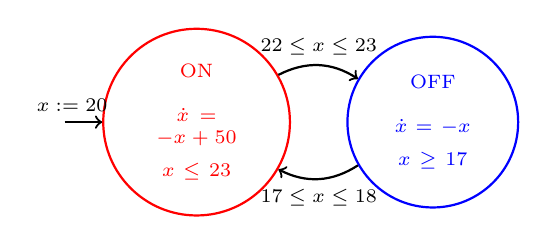
\begin{tikzpicture}[scale=0.6]
  \node[draw, circle, text width = 1.4cm, text centered, thick,color=red] (l1) at (0,0) {\scriptsize{ON\\ \ \\$\dot{x}=-x+50$\\ $x\leq 23$}};
  \node[draw, circle, text width = 1.4cm, text centered, color=blue, thick] (l2) at (5,0) {\scriptsize{OFF\\ \ \\$\dot{x}=-x$\\ $x\geq 17$}};
  \path[thick,->] (l1) edge[bend left] node[above] {\scriptsize{$22\leq x\leq 23$}} (l2);
  \path[thick,->] (l2) edge[bend left] node[below] {\scriptsize{$17\leq x\leq 18$}} (l1);
  \node (dummy) at (-3,0) {};
  \path[thick,->] (dummy) edge node[pos=0.2, above] {\scriptsize{$x:=20$}} (l1);
 \end{tikzpicture}
 \end{column}
 \begin{column}{5cm}
 \begin{tikzpicture}[scale=0.4]
  \thermostatcon{0}{0};
 \end{tikzpicture}
\end{column}
\end{columns}
A state = a discrete state + a valuation for the variables.
\end{center}

\end{frame}

\subsection{Model checking of an hybrid automaton}
\begin{frame}{The reachability analysis}
There are several methods to ensure the safety of an hybrid automaton:
\begin{itemize}
\item theorem proving;
\item interval based methods;
\item flowpipe computation.
\end{itemize}

\begin{figure}
\includegraphics[width=0.5\columnwidth]{images/zono.png}
An example of a flowpipe.
\end{figure}

\end{frame}

\begin{frame}[t]{Two definitions of polyhedra}
Key issue for flowpipe computation: being able to manipulate these polyhedra. There are two definitions for polyhedra:
\only<2,3>{\begin{block}{$\mathcal{V}$-polyhedron}
A $\mathcal{V}$-polyhedron $P$ is the Minkowsky sum of the convex hull of a set $V$ of vertices and the conic hull of a set $C$ of vectors. $P= conv(V) + cone(C)$.
\end{block}}
\only<3>{
\begin{figure}
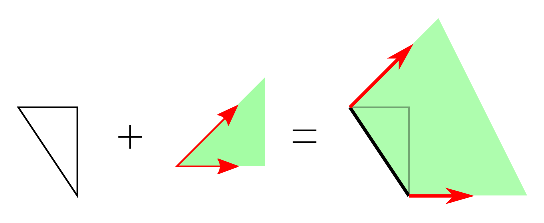
\includegraphics[scale=1]{images/vpoly.eps}\\
Construction of a $\mathcal{V}$-polytope
\end{figure}
}
\begin{itemize}
\visible<4->{\item the $\mathcal{V}$-polyhedron;}
\visible<6->{\item the $\mathcal{H}$-polyhedron.}
\end{itemize}
\only<4,5>{\begin{block}{$\mathcal{H}$-polyhedron}
An $H$-polyhedron $P$ is the intersection of a set of half-spaces: $\cap_{i=0}^n\{ x|a_i.x\leq b_i \}$. This can be written with a matrix $\{ x| Ax \leq b\}$.
\end{block}}
\only<5>{
\begin{figure}
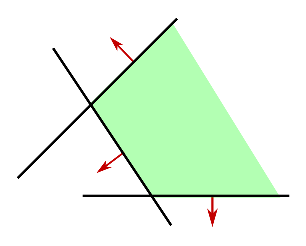
\includegraphics[scale=0.7]{images/hpoly.eps}\\
Construction of a $\mathcal{H}$-polytope
\end{figure}
}
\only<6>{
\begin{figure}
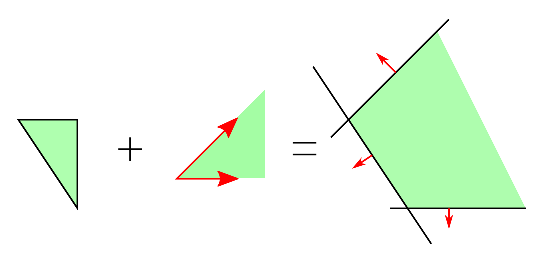
\includegraphics[scale=0.7]{images/poly.eps}\\
$\mathcal{H}$ and $\mathcal{V}$ representations are equivalent.
\end{figure}
}
\visible<7,8>{
\begin{table}
\centering
\begin{tabular}{| c | c | c | c |}
	\hline	
		    & $.\ \cap\ .$ & $.\ \cup\ .$ & $.\ +\ .$ \\ \hline
	$\mathcal{V}$-Polyhedra   & $-$ & $+$ & $+$ \\ \hline
   	$\mathcal{H}$-Polyhedra   & $+$ & $-$ & $-$\\ \hline
\end{tabular}\\
\vspace*{0.1cm}
Comparison of the two representations.
\end{table}
\vspace*{-0.1cm}
}

%\visible<7,8>{\begin{block}{Central theorem of polyhedra representation}
%A subset $P$ of $\mathbb{R}^d$ is a $\mathcal{V}$-polyhedron if and only if it is an $\mathcal{H}$-polyhedron.
%\end{block}}
\visible<8>{The internship resulted in a contribution to HyPro.}
\end{frame}

\begin{frame} 
	\begin{center}{\Large Plan }\end{center}
	\tableofcontents
\end{frame}





